\documentclass{examen}

\begin{document}
\modulo{Lenguajes de marcas y sistemas de gesti�n de informaci�n}

\pregunta{Dado el archivo XML que se puede encontrar al final, 
crear una hoja de estilo XSLT que genere el HTML necesario para que se extraigan en forma de tabla el precio y la cantidad de memoria de todos los dispositivos
}{4}


\begin{figure}[h]
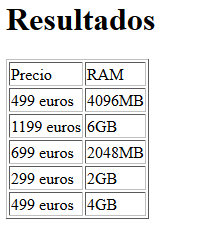
\includegraphics[scale=0.8]{examen-img/ejtabla.png}
\end{figure}


\pregunta{Transformar el XML del pedido en el XML que se muestra al final. Los productos se han clasificado en ``caros'' y ``baratos'. Un producto cualquiera se considera caro si cuesta m�s de 500 y baratos si vale menos. Observa adem�s que todas las unidades van en GB y que los precios se han convertido en atributos. En los port�tiles no aparece el tipo de disco. En las tablets no aparece en el resultado ni el tama�o ni la bater�a.}{6}

\break

\begin{lstlisting}{language=xml}
<!--FICHERO ORIGINAL-->
<pedido>
	<portatiles>
		<portatil>
			<peso>1430</peso>
			<ram unidad="MB">4096</ram>
			<disco tipo="ssd">500</disco>
			<precio>499</precio>
		</portatil>
		<portatil>
			<peso>1830</peso>
			<ram unidad="GB">6</ram>
			<disco tipo="ssd">1000</disco>
			<precio>1199</precio>
		</portatil>
		<portatil>
			<peso>1250</peso>
			<ram unidad="MB">2048</ram>
			<disco tipo="ssd">750</disco>
			<precio>699</precio>
		</portatil>
	</portatiles>
	<tablets>
		<tablet>
			<plataforma>Android</plataforma>
			<caracteristicas>
				<memoria medida="GB">2</memoria>
				<tamanio medida="pulgadas">6</tamanio>
				<bateria>LiPo</bateria>
			</caracteristicas>
			<precio>299</precio>
		</tablet>
		<tablet>
			<plataforma>iOS</plataforma>
			<caracteristicas>
				<memoria medida="GB">4</memoria>
				<tamanio medida="pulgadas">9</tamanio>
				<bateria>LiIon</bateria>
			</caracteristicas>
			<precio>499</precio>
		</tablet>
	</tablets>
</pedido>

\end{lstlisting}

\break

\begin{lstlisting}{language=xml}
<!--Fichero que debe salir como resultado del ejercicio 2-->
<pedido>
	<caros>        
            <portatil precio="1199">
                    <peso>1830</peso>
                    <ram cantidad="6" unidad="GB"/>
            </portatil>
            <portatil precio="699">
                    <peso>1250</peso>
                    <ram cantidad="2" unidad="GB"/>
            </portatil>
        </caros>
        <baratos>
            <portatil precio="499">
                    <peso>1430</peso>
                    <ram cantidad="4" unidad="GB"/>
            </portatil precio="299">
            <tablet precio="299">
                    <plataforma>Android</plataforma>
                    <caracteristicas>
                            <memoria cantidad="2" medida="GB"/>
                    </caracteristicas>
            </tablet>
            <tablet precio="499">
                    <plataforma>iOS</plataforma>
                    <caracteristicas>
                            <memoria cantidad="4" medida="GB"/>
                    </caracteristicas>
            </tablet>
    </baratos>
</pedido>

\end{lstlisting}


\end{document}
